\documentclass[t,aspectratio=1610]{beamer}

\usepackage{bxcjkjatype}
\usepackage{listings}
\usepackage{tikz}
\newcounter{row}
\newcounter{col}

\newcommand\setrow[9]{
  \setcounter{col}{1}
  \foreach \n in {#1, #2, #3, #4, #5, #6, #7, #8, #9} {
    \edef\x{\value{col} - 0.5}
    \edef\y{9.5 - \value{row}}
    \node[anchor=center] at (\x, \y) {\n};
    \stepcounter{col}
  }
  \stepcounter{row}
}

\usetheme{default}
\beamertemplatenavigationsymbolsempty\setbeamersize{
    text margin left=0.75cm,
    text margin right=0.75cm
}

% Title
\setbeamerfont{title}{size=\LARGE, 
                      series=\bfseries,
                      family=\rmfamily}
\setbeamercolor{title}{fg=blue!70!black}
\setbeamertemplate{frametitle}{
    \nointerlineskip\;
    \begin{beamercolorbox}[sep=.1ex,
                           wd=\paperwidth,
                           leftskip=0.5cm,
                           rightskip=0pt]{frametitle}
        \usebeamerfont{frametitle}
        \usebeamercolor[fg]{frametitle}
        \\
        \hfill
        \insertfrmetitle\;
        \strut\;
    \end{beamercolorbox}
}
% Alerted text
\setbeamerfont{alerted text}{shape=\itshape,
                             series=\bfseries}
\setbeamercolor{alerted text}{fg=black!90}
% Itemize
\setbeamercolor{itemize item}{fg=black!90}
\setbeamercolor{itemize subitem}{fg=black!90}
\setbeamertemplate{itemize item}[circle]
\setbeamertemplate{itemize subitem}[triangle]
% Blocks
\setbeamercolor{block body example}{fg=black!90,
                                    bg=black!10}
\setbeamercolor{block title example}{fg=white,
                                     bg=blue!30!black!30}
\setbeamertemplate{blocks}[shadow=true]

\title{Hurray! It's Theory of Computation}
\subtitle{\Large{SAT Sudoku}}
\author{Bevilacqua Joey \\ De Vita Gianmarco \\ Luini Alessandro\\ Maggioni Claudio}
\institute{Universit\`a della Svizzera Italiana\\ Faculty of Informatics\\ \href{http://www.unisi.ch}{www.unisi.ch}}
\date{May 26, 2021}

\begin{document}
{
\usebackgroundtemplate{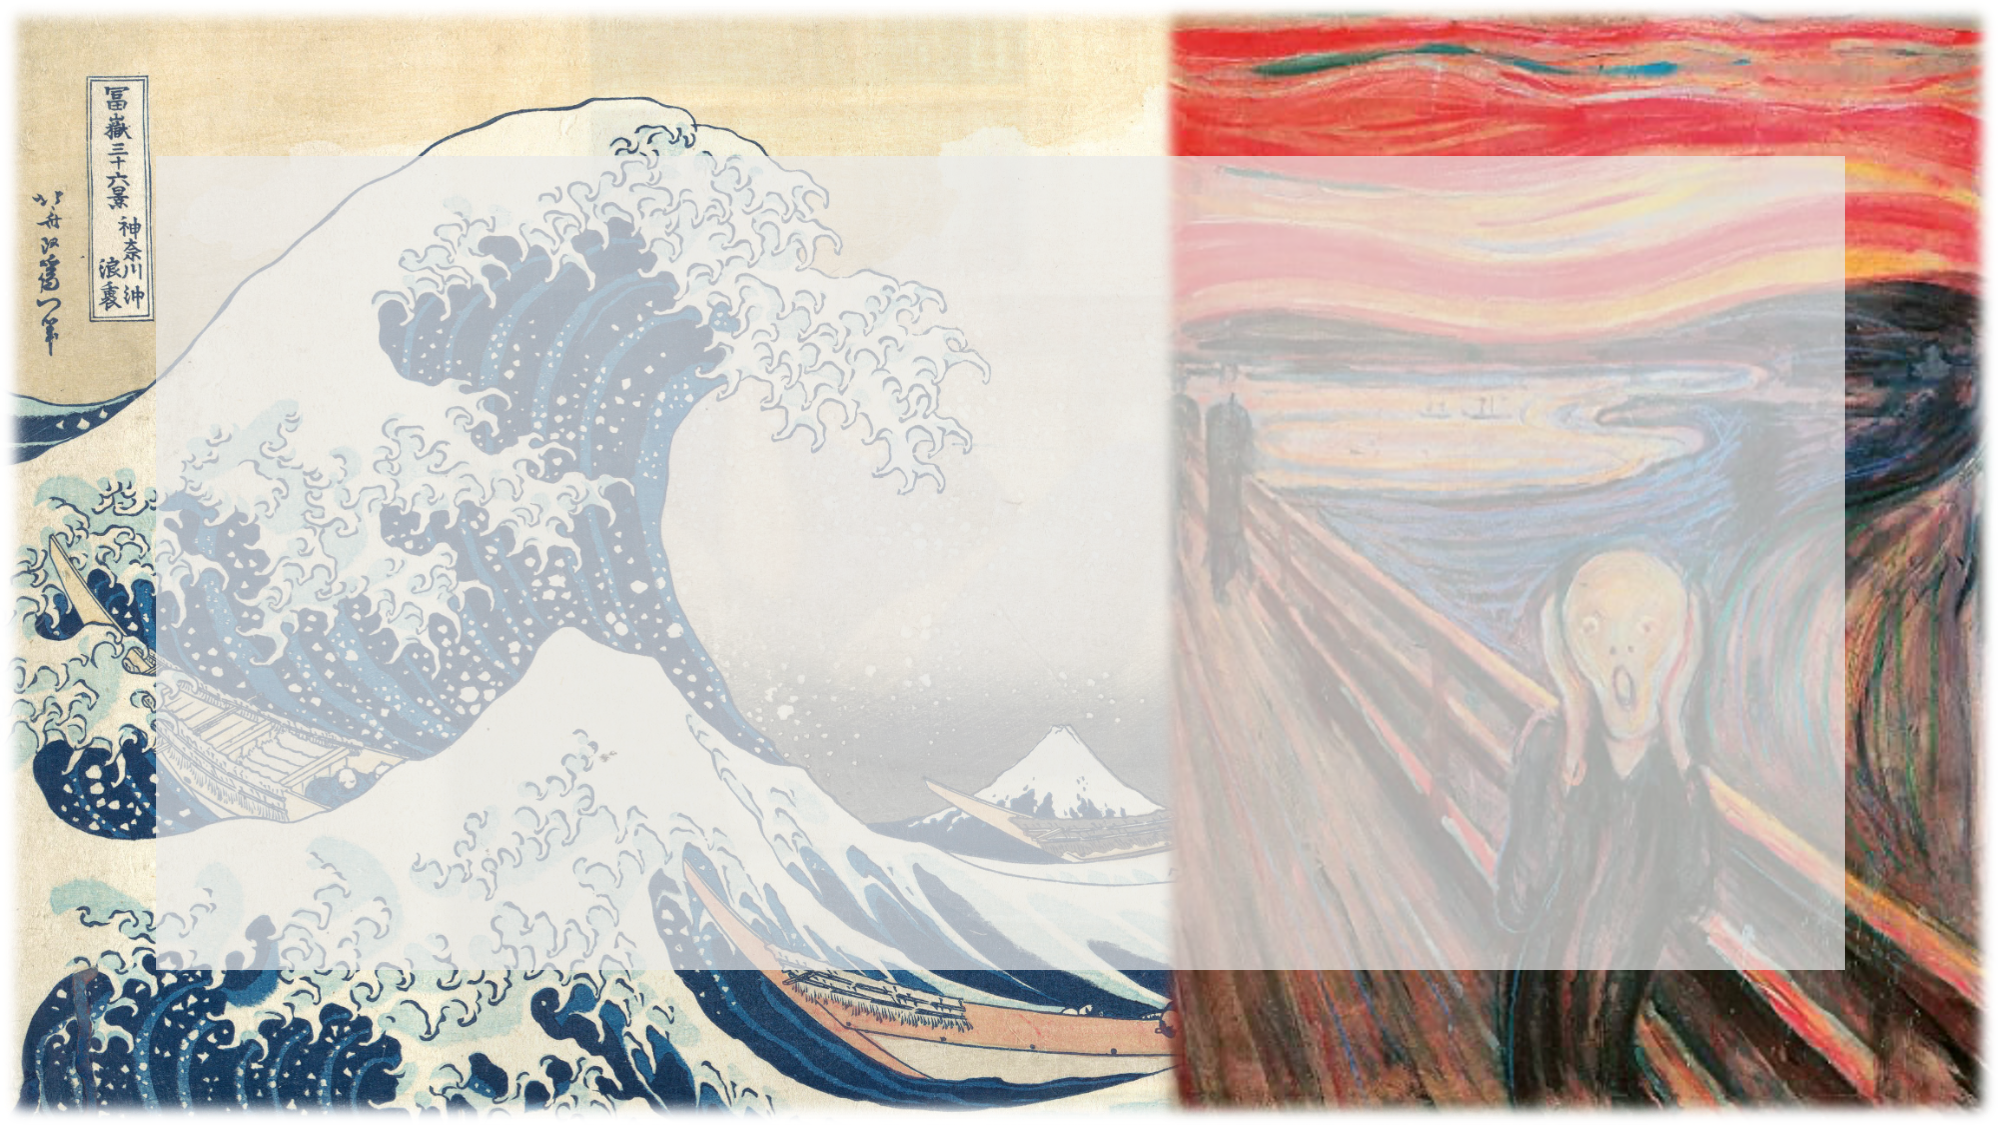
\includegraphics[width=1\paperwidth, height=1\paperheight]{screamc}}%
\begin{frame}
\maketitle
\end{frame}
}

\begin{frame}
\begin{figure}[h]
\begin{center}
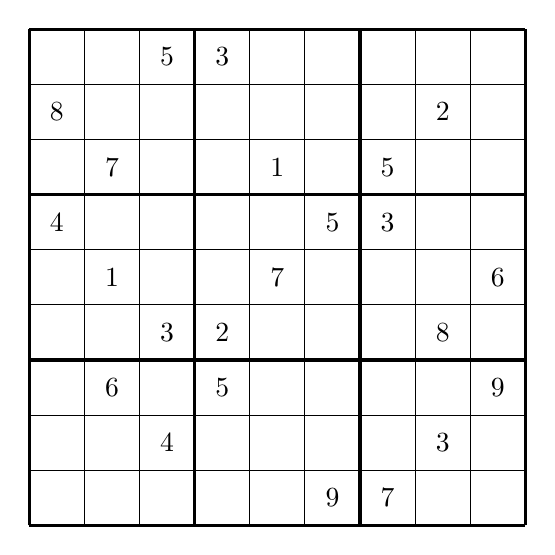
\begin{tikzpicture}[scale=.7]
  \begin{scope}
    \draw (0, 0) grid (9, 9);
    \draw[very thick, scale=3] (0, 0) grid (3, 3);

    \setcounter{row}{1}
    \setrow { }{ }{5}  {3}{ }{ }  { }{ }{ }
    \setrow {8}{ }{ }  { }{ }{ }  { }{2}{ }
    \setrow { }{7}{ }  { }{1}{ }  {5}{ }{ }
    \setrow {4}{ }{ }  { }{ }{5}  {3}{ }{ }
    \setrow { }{1}{ }  { }{7}{ }  { }{ }{6}
    \setrow { }{ }{3}  {2}{ }{ }  { }{8}{ }
    \setrow { }{6}{ }  {5}{ }{ }  { }{ }{9}
    \setrow { }{ }{4}  { }{ }{ }  { }{3}{ }
    \setrow { }{ }{ }  { }{ }{9}  {7}{ }{ }
  \end{scope}
\end{tikzpicture}
\end{center}
\caption{A $9\times 9$ Sudoku puzzle.}
\end{figure}
\end{frame}

\begin{frame}
\textbf{Sudoku} \\

Although Sudoku is a Japanese word (\begin{uCJK}\UTF{6570}\UTF{72EC}\end{uCJK} – ``single digit''),
Some sources state it was invented by the famous Swiss mathematician Euler.
However, it is generally acknowledged that the origin of this game is European
(around XIX century) and that the modern and common version has been realized
in the US in the second half of the XX century named as ``Number Place''.
\end{frame}

\begin{frame}
\begin{figure}[h]
\begin{center}
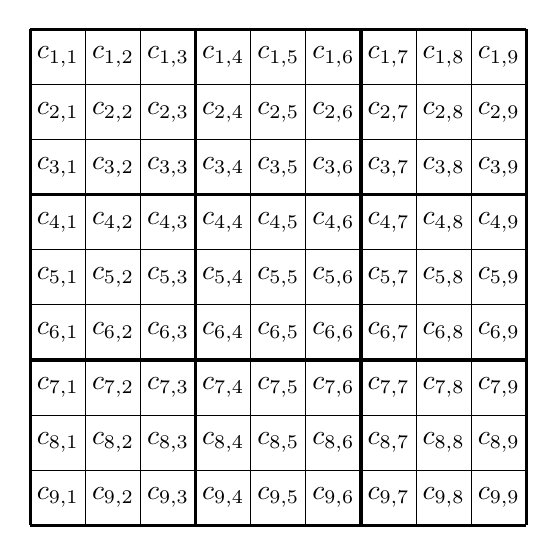
\begin{tikzpicture}[scale=.7]
  \begin{scope}
    \draw (0, 0) grid (9, 9);
    \draw[very thick, scale=3] (0, 0) grid (3, 3);

    \setcounter{row}{1}
    \foreach \i in {1,...,9}
    {
    \setrow {$c_{\i,1}$ }{$c_{\i,2}$}{$c_{\i,3}$}  {$c_{\i,4}$}{$c_{\i,5}$}{$c_{\i,6}$}  {$c_{\i,7}$}{$c_{\i,8}$}{$c_{\i,9}$}
    }
  \end{scope}
\end{tikzpicture}
\end{center}
\caption{A $9\times 9$ Sudoku puzzle.}
\end{figure}
\end{frame}

\begin{frame}
KTHXBYE
\end{frame}

{
\usebackgroundtemplate{
    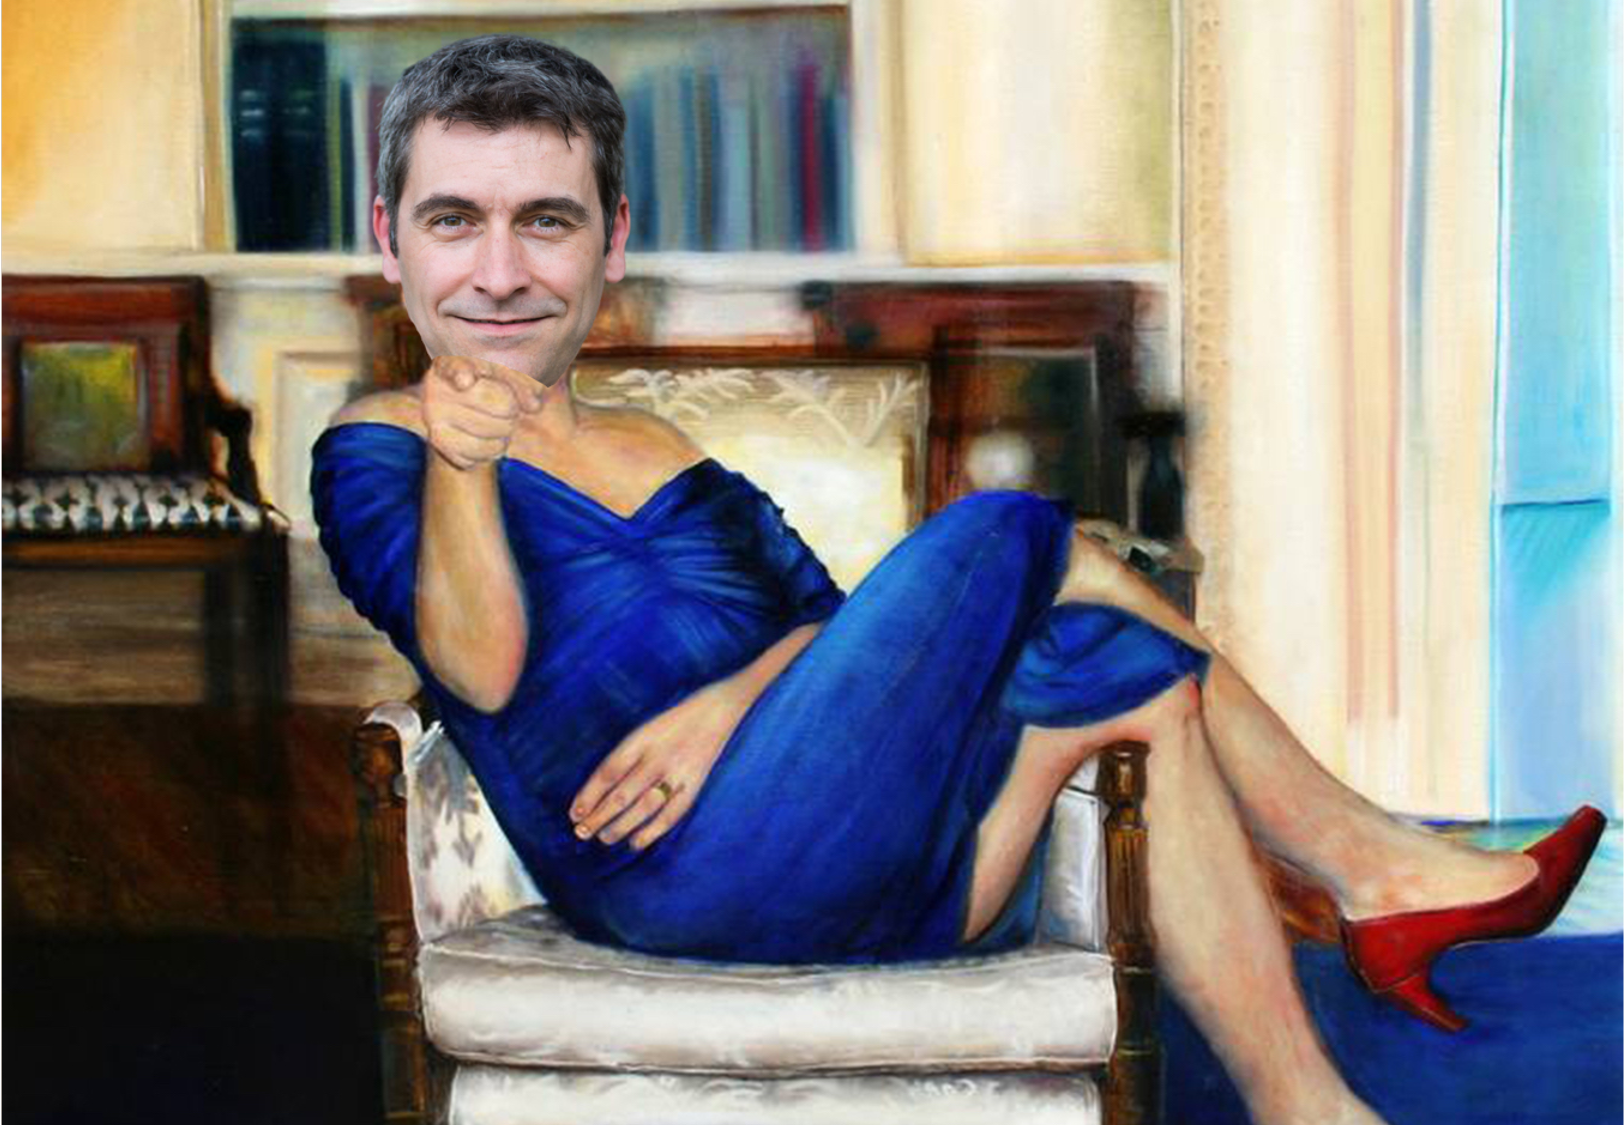
\includegraphics[width=1\paperwidth, height=1\paperheight]{end.png}
}
\begin{frame}
\end{frame}
}

\end{document}